\documentclass[times,10pt,twocolumn]{article}
\usepackage{ipdps}
\usepackage{vmargin}
\setpapersize{USletter}
\setmargnohf{0.8125in}{1in}{6.875in}{8.875in}
\pagestyle{empty}
\newenvironment{twoaffiliations}{\begin{tabular}{cc}}{\end{tabular}}
\newenvironment{oddaffiliation}{\begin{center}}{\\~\\\end{center}}
%\documentclass[times,11pt,onecolumn]{article} 
%\usepackage{latex8}
%\usepackage{times}
\usepackage{epsfig}
%\pagestyle{empty}
%\newcommand{\mt}[1]{\mbox{#1}}

\title{MPEG-2 Decoding in a Stream Programming Language}

\author{
  Matthew Drake, Hank Hoffmann, Rodric Rabbah, and Saman Amarasinghe\\
  \begin{twoaffiliations}
    Massachusetts Institute of Technology\\
    Computer Science and Artificial Intelligence Laboratory\\
    \{madrake, hank, rabbah, saman\}@mit.edu
  \end{twoaffiliations}
}

\begin{document}
  
  \maketitle
  \thispagestyle{empty}
  
  \begin{abstract}
    Applications that are structured around some notion of a "stream"
are becoming increasingly important and widespread.  There is
evidence that streaming media applications are already consuming
most of the cycles on consumer machines \cite{Rix98}, and their
use is continuing to grow.  {\StreamIt} is a language and compiler
specifically designed for modern stream programming.  Despite the
prevalence of these applications, there is surprisingly little
language and compiler for practical, large-scale stream
programming.  {\StreamIt} is a language and compiler specifically
designed for modern stream programming.  The {\StreamIt} langauge
holds two goals: first, to provide high-level stream abstractions
that improve programmer productivity and program robustness within
the streaming domain; second, to serve as a common machine
language for grid-based processors.  At the same time, {\StreamIt}
compiler aims to perform stream-specific optimizations to achieve
the performance of an expert programmer.  This thesis develops
several techniques for scheduling execution of {\filters} in
{\StreamIt}.  The work focuses on correctness as well as
minimizing buffering requirements and stored schedule size.

  \end{abstract}
  
  \section{Introduction}

The domain of stream programs is important because it stands at the
intersection of trends in applications and architectures.  Stream
programming naturally represents applications such as audio, video,
digital signal processing, and data analysis; applications that are
increasing prevalent as computing moves towards data-centric
applications and to the mobile and embedded space.  Also, by virtue of
their structure -- a graph of independent computational nodes (termed
{\it filters}) with explicit and regular communication -- stream
programs are a natural fit for exploiting coarse-grained parallelism
suitable for multicore architectures.  The interest in streaming
applications has spawned a number of streaming languages that target
the streaming domain, including StreamIt~\cite{streamitcc},
Brook~\cite{brook04}, Cg~\cite{cg03},
SPUR~\cite{spur05samos}, Spidle~\cite{spidle03}, Lime~\cite{lime10},
and SPL~\cite{spl09}.

In a stream program, filters define an atomic execution step that
repeats for many iterations; each execution step discards a number of
data items from filter's input edge.  Often, a filter does not discard
all the data items that it read for the current execution step,
requiring these inspected (but not discarded) items for a future
iteration (or iterations) of the filter.  This type of filter is
described as performing a sliding window computation on its
input. Sliding window computations are prevalent in stream programs.
Examples of sliding window computations include FIR filters; moving
averages and differences; error correcting codes; motion estimation;
and network packet inspection.  A recent study of a large streaming
benchmark suite written in the StreamIt programming language finds
that 17 of the 30 real-world benchmarks include at least one filter
that performs a sliding window computation~\cite{streamit-suite}.


Figure~\ref{fig:fir-nopeeking} shows how to perform a sliding
window FIR filter via state carried between iterations of a filter.
This implementation is difficult for the compiler to analyze and
reason about.  Some programming languages (e.g., Brook, Lime,
StreamIt, and IBM SPL) go so far as to include idioms that directly
represent sliding window computation, allowing the programmer to
specify, for each filter, the size of the window and the number of
items discarded after an execution of the filter.
Figure~\ref{fig:fir-peeking} shows how language extensions of the
StreamIt programming language elegantly expose sliding windows for
compiler analysis and optimization.

A goal of stream programming is to directly expose to the software
layer the necessary information to enable automatic management of
coarse-grained parallelism.  Stream programs expose multiple forms of
parallelism: pipeline parallelism that exists between producers and
consumers; task parallelism that exists between pairs of filters on
parallel branches of the stream graph; and data parallelism that
exists when a filter is stateless and can thus be replicated.  Data
parallelism is the most attractive, as it provides load-balanced and
limitless parallelism (as long as input data is available).  A filter
that is stateful, and cannot be data-parallelized, becomes a limit to
parallelization scalability, as the work of that filter cannot be
divided; the most load-intensive stateful filter becomes a
bottleneck.

This paper presents a compiler framework for data-parallelizing
filters that perform sliding window computations when the properties
of the sliding window can be calculated statically.  If sliding window
filters required state, this state would represent a new
parallelization bottleneck.  Sliding windows are the bottleneck in 11
of the 17 real-world benchmarks in the StreamIt Benchmark Suite that
contain sliding windows~\cite{streamit-suite}.  For example, examining
the Channelvocoder benchmark, this state would limit scalability to 18
cores, whereas our techniques scale to at least 64 cores.

Data-parallelizing a filter is performed via a transformation termed
{\it fission} (verb form {\it fiss})~\cite{streamit-asplos}.  Fission
is the process of data-parallelizing a stateless filter by duplicating
the filter a certain number of ways, assigning duplicates to distinct
cores, and correctly distributed input data to and collecting output
data from the duplicates.  The duplicated filters are referred to as
{\it products}.  When a sliding window is present, fission is
accomplished by duplicating certain input items since they are
required by multiple products.  This duplication translates into
inter-core communication, a limiting factor for scalability when
targeting multicore architectures.

Previous approaches duplicate each input data item to all products,
with products ignoring (decimating) items that are not
needed~\cite{streamit-asplos}.  We will show that this strategy limits
scalability for multicores by requiring too much inter-core
communication.  In contrast, our strategy precisely routes each input
item to the minimal set of product filters that requires the item.
Unlike previous work, our techniques are defined on
multiple input and multiple output filters, removing the need to
introduce synchronization filters that serialize data before and
after the product filters.  

Our techniques operate on {\it static-rate} stream graphs, meaning
that the number of items produced, the number of items consumed, and
the number of items inspected by each filter can be determined
statically.  Because of this property, a steady-state schedule of
filter firings can be calculated that does not grow buffers and can be
executed indefinitely~\cite{lee87}.  Our techniques are conscious of
the spatial locality between producers and consumers.  Our framework
includes techniques that can determine when spatial locality can be
increased by altering the steady-state schedule.  When applicable, our
techniques can reduce the overall sharing (and thus inter-core
communication) requirement to below a threshold percent of the total
input communication for each sliding window filter that is
data-parallelized. 

\begin{figure}[t]
\centering
\subfigure[]{\includegraphics[width=3.3in]{figures/fir-nopeeking.pdf}\label{fig:fir-nopeeking}}
\subfigure[]{\includegraphics[width=3.3in]{figures/fir-peeking.pdf}\label{fig:fir-peeking}}
\caption[Two implementations of an FIR filter.]{\label{fig:fir-code}
  Two StreamIt implementations of an FIR filter:
   (a) the non-peeking version implemented via a
  stateful circular buffer; and (b) the peeking version. Only steady-state implementation is
  given.}
\end{figure}

The framework presented is defined on a model of computation that is
agnostic of source language.  To evaluate our techniques we have
implemented them in the context of the StreamIt compiler
infrastructure~\cite{gordon-asplos06}.  Our transformations are guided
by the parallelization management techniques presented
in~\cite{gordon-asplos06}.  We employ 3 real-world benchmarks from the
StreamIt Benchmark Suite~\cite{streamit-suite} that include sliding
window computation.  We demonstrate the effectiveness of our
techniques by comparing them to previously published techniques on 2
multicore architectures: a 16-core SMP shared-memory multicore and the
64-core distributed-memory Tilera TILE64.  We show that
our techniques are required to achieve scalable parallelization on
both architectures, achieving a 6.7x mean speedup on the 16-core SMP
and a 1.8x mean speedup on the 64-core distributed memory multicore
over a previously published technique.

\subsection{Contributions}
This paper makes the following contributions:
\begin{itemize}
  % \myitem{Motivation for Exposing Sliding Windows in Stream
  %   Languages}: Without exposing sliding windows in the language, it
  % requires heroic effort by the compiler to analyze the access patterns
  % of such a filter. Without success, the compiler will not be able to
  % data-parallelize these filters.  This will prevent robust 
  % parallelization scalability for streaming applications.

  \myitem{Generalized Fission of Sliding Window Filters}: We present a
  transformation that fisses sliding window filters with multiple
  input and multiple outputs.  The technique also supports filters
  that with multiple schedules of execution.  General fission defines
  a precise pattern of communication of input data to the products
  that can be reasoned upon by our other techniques.

  \myitem{Sharing Reduction}: We are the first to present a technique
  that decides when it is possible to decrease the amount of sharing
  between fission products by altering the steady-state of a stream
  graph, thus decreasing inter-core communication.  The technique
  reasons about all the sliding window filters of the stream graph,
  and when possible, reduces the sharing requirement to below a given
  threshold percent of the total input of the filters. 

  \myitem{Data Parallelization of Stream Graph}: We present a
  framework for data-parallelizing all of the filters of a stream
  graph employing the fission transformation on individual filters and
  applying sharing reduction when possible.  This framework optimizes
  for spatial locality and enables the compiler to automatically and
  effectively manage parallelization across varying multicore
  architectures.

  \myitem{Enable Robust Parallelization Scaling for Multicores}: For
  streaming applications with sliding window computation, previously
  published data-parallelization transformations do not scale for our
  target multicores. Our techniques enable robust parallelization
  scalability by reducing inter-core communication.  We achieve a 17x
  mean parallelization speedup for a 16-core SMP and a 62.3x mean
  parallelization speedup for the 64-core TILE64 across our benchmarks.

\end{itemize}

% \begin{figure}[t]
% \centering
% \begin{subfloat}
% \begin{minipage}[b]{0.45\textwidth}
% \eightpoint
% \begin{verbatim}
% float->float filter FIR(int N) {
%   int srcBuffer[N];
%   int srcEnd = 0; 
%   ...
%   work push 1 pop 1 {
%     srcBuffer[srcEnd] = pop();
%     float sum = 0;
%     for (int i=0; i<N; i++) {
%       sum += weights[i] * srcBuffer[(srcEnd + i + 1) % N];
%     }
%     push(sum);
%     srcEnd = (srcEnd + 1) % N;
%   }
% }
% \end{verbatim}
% \vspace{-8pt}
% \end{minipage}%
% \caption{ \label{fig:fir-nopeeking}}
% \end{subfloat}%
% \qquad
% \begin{subfloat}
% \begin{minipage}[b]{0.45\textwidth}
% \eightpoint
% \begin{verbatim}
% float->float filter FIR(int N) {
%   ...
%   work push 1 pop 1 peek N {
%     float sum = 0;
%     for (int i=0; i<N; i++) {
%       sum += weights[i] * peek(i);
%     }
%     push(sum);
%     pop();
%   }
% }
% \end{verbatim}
% \vspace{-18pt}
% \end{minipage}
% \caption{ \label{fig:fir-streamit}}
% \end{subfloat}
% \caption[Two implementations of an FIR filter.]{\label{fig:fir-code}
%   Two StreamIt implementations of an FIR filter:
%    \subref{fig:fir-nopeeking} the non-peeking version implemented via a
%   stateful circular buffer; and \subref{fig:fir-streamit} the peeking version. Only steady-state implementation is
%   given.}
% \end{figure}

  \Section{MPEG-2 Video Coding and Decoding}

MPEG-2~\cite{MPEG2} is a popular coding and decoding standard
for digital video data. The scheme is a subset of both the
DVD-Video~\cite{DVDVideo} standard for storing movies, and the Digital
Video Broadcasting specifications for transmitting HDTV and
SDTV~\cite{DVB}. The scheme is used by a wide variety of multimedia
applications and appliances such as the Tivo Digital Video
Recorder~\cite{tivo}, and the DirecTV satellite broadcast
service~\cite{directv}.

MPEG-2 encoding uses both {\it lossy} compression and {\it lossless}
compression. Lossy compression permanently eliminates information from
a video based on a human perception model. Humans are much better at
discerning changes in color intensity (luminance information) than
changes in color (chrominance information). Humans are also much more
sensitive to low frequency image components, such as a blue sky, than
to high frequency image components, such as a plaid shirt. Details
which humans are likely to miss can be thrown away without affecting
the perceived video quality.

Lossless compression eliminates redundant information while allowing
for its later reconstruction. Similarities between adjacent video
pictures are encoded using motion prediction, and all data is Huffman
compressed\cite{Huffman52}. The amount of lossy and lossless
compression depends on the video data. Common compression ratios range
from 10:1 to 100:1. For example, HDTV with a resolution of 1280x720
pixels and a streaming rate of 59.94 frames per second, has an
uncompressed data rate of 1.33 Gigabits per second. It is compressed at 
an average rate of 66:1, reducing the required streaming rate to
20 Megabits per second~\cite{imagevidstandards, Page 3}.

\SubSection{MPEG Coding}

\begin{figure}[t]
\begin{center}
\vspace{-12pt}
% \framebox{
% \includegraphics[scale=1, angle=0]{./mpeg-encoder.eps}
%}
% \vspace{-6pt}
% \nocaptionrule
 \caption{MPEG encoder.}
 \label{fig:mpeg-encoder}
%\vspace{-18pt}
\end{center}
\end{figure}

An overview of the encoding process is illustrated in
Figure~\ref{fig:mpeg-encoder}. The encoder operates on a sequence of
pictures. Each picture is made up of pixels arranged in a 16x16 array
known as a macroblock. Macroblocks are formed from 8x8 arrays, 
known as blocks, which contain pixel data for a single color channel. 
Each color channel in a macroblock may be represented by a 2x2 matrix
of blocks, or downsampled to a 1x2 or 1x1 block representation.
The compression in MPEG is achieved largely via motion estimation, which
detects and eliminates similarities between macroblocks across
pictures. Specifically, the motion estimator calculates a motion
vector to represent the horizontal and vertical displacement of a
given macroblock (i.e., the one being encoded) to a matching
macroblock-sized area in a reference picture. 
The matching macroblock is removed (subtracted) from the
current picture on a pixel by pixel basis. The result is a residual
predictive-code (P) picture. It represents the difference between the
current picture and the reference picture. Reference pictures encoded without
the use of motion prediction are intra-coded (I) pictures. In addition to forward
motion prediction, it is possible to encode new pictures using motion
estimation from both previous and subsequent pictures. Such pictures
are bidirectionally predictive-coded (B) pictures, and they exploit a
greater amount of temporal locality.

Each of the I, P, and B pictures then undergoes a 2-dimensional
discrete cosine transform (DCT) which separates the picture into parts
with varying visual importance. The input to the DCT is one block. 
The output of the
DCT is an 8x8 matrix of frequency coefficients. The upper left corner
of the matrix represents low frequencies, whereas the lower right
corner represents higher frequencies. The latter are often small and
can be neglected without sacrificing human visual perception.

\begin{figure}[t]
\begin{center}
\vspace{-12pt}
% \framebox{
% \includegraphics[scale=1, angle=0]{./zigzag.eps}
%}
% \vspace{-6pt}
% \nocaptionrule
 \caption{Zig-Zag scan patterns.}
 \label{fig:zigzag}
%\vspace{-18pt}
\end{center}
\end{figure}

The DCT coeffecients are quantized to reduce the number of bits needed
to represent them. Following quantization, many coefficients are
effectively reduced to zero. The DCT matrix is then run-length
encoded by emitting each non-zero coefficient, followed by the number
of zeros that precede it, along with the number of bits needed to
represent the coefficient, and its value. The run-length encoder
scans the DCT matrix in a zig-zag order (Figure~\ref{fig:zigzag}) to
consolidate the zeros in the matrix.

Finally, the output of the run-length encoder, motion vector data,
and other information (e.g., type of picture), are Huffman coded to 
further reduce the average number of bits per data item. The compressed
stream is sent to the output device.

\SubSection{MPEG Decoding}

An MPEG-2 input stream is organized as a Group of Pictures (GOP)
which contains all the information needed to reconstruct a video. The
GOP contains the three kinds of pictures produced by the encoder,
namely I, P, and B pictures. I pictures are intended to assist scene
cuts, random access, fast forward, or fast reverse
playback~\cite{MPEG2, Page 14 6.1.1.7}. A typical I:P:B picture ratio
in a GOP is 1:3:8, and a typical picture pattern is a
repetition of the following sequence: I~B~B~P~B~B~P~B~B~P~B~B. The
input pictures are not ordered temporally within the stream. Rather,
they are ordered such that if a decoder encounters a P picture, its
motion prediction is with respect to the previously decoded I or P
picture, and if the decoder encounters a B picture, its motion
prediction is with respect the previously two decoded I or P pictures.

As with the encoding process, pictures are divided up into 16x16 pixel
macroblocks, themselves composed of 8x8 blocks. Macroblocks
specify colors using a {\it luminance} channel to represent saturation
(color intensity), and two {\it chrominance} channels to represent
hue. MPEG-2 streams specify a chroma format which allows the
chrominance data to be sampled at a lower rate. The most common chroma 
format is 4:2:0 which represents a macroblock using four blocks for the
luminance channel and one block for each of the two chrominance
channels. 

\begin{figure}[t]
\begin{center}
\vspace{-12pt}
% \framebox{
% \includegraphics[scale=1, angle=0]{./mpeg-decoder.eps}
%}
% \vspace{-6pt}
% \nocaptionrule
 \caption{MPEG decoder.}
 \label{fig:mpeg-decoder}
%\vspace{-18pt}
\end{center}
\end{figure}

The decoding process is illustrated in
Figure~\ref{fig:mpeg-decoder}. It is conceptually the reverse of the
encoding process. The input stream is Huffman and run-length decoded,
resulting in quantized DCT matrices. The DCT coefficients are scaled
in magnitude and an inverse DCT (IDCT) maps the frequency matrices to
the spatial domain.

Finally, the motion vectors parsed from the data stream are passed to
a motion compensator, which reconstructs the orginal pictures. In the
case of I pictures, the compensator need not make any changes since
these pictures were not subject to motion estimation~\footnote{I 
pictures are allowed to contain concealment motion vectors which aid in
macroblock reconstruction should a bitstream error destroy the 
frequency coefficient data. We ignore this special case.}. In the case of P
and B pictures however, motion vectors are used to find the
corresponding region in the current reference pictures. The
compensator then adds the relevant reference macroblocks to the
current picture to reconstruct it. These pictures are then emitted to
an output device.
  \Section{StreamIt Programming Language}
\label{sec:streamit}

StreamIt~\cite{streamit-cc} is an architecture independent language
that is designed for stream programming. In StreamIt, programs are
represented as graphs where nodes represent computation and edges
represent FIFO-ordered communication of data over tapes. The language
features several novelties that are essential for large scale program
development. The language is modular, parameterizable, malleable and
architecture independent. In addition, the language exposes the
inherent parallelism and communication patterns that are prevalent in
streaming programs.

\begin{figure*}[t]
  \begin{minipage}[t]{4.0in}
    {
	\begin{scriptsize}
	  \begin{verbatim}
	    int->int filter ZigZagScan(int N, int[N] Order)
	    {
	        work pop N push N {
	        for (int i = 0; i < N; i++) {
	          int pixel = peek(Order[i]);
	          push(pixel);
	        }
	        for (int i = 0; i < N; i++) {
	          pop();
	        }
	      }
	    }
	  \end{verbatim}
	\end{scriptsize}
    }
    % \vspace{-3pt}
    \caption{Example filter implementing zig-zag scanning.}
    % \label{fig:zigzag-filter}
  \end{minipage}
  ~~\vrule~~
  \begin{minipage}[t]{3.0in}
    {  
	\begin{scriptsize}
	  \begin{verbatim}
	    int[64] Ordering = 
	      {00, 01, 05, 06, 14, 15, 27, 28,
	       02, 04, 07, 13, 16, 26, 29, 42,
	       03, 08, 12, 17, 25, 30, 41, 43,
	       09, 11, 18, 24, 31, 40, 44, 53,
	       10, 19, 23, 32, 39, 45, 52, 54,
	       20, 22, 33, 38, 46, 51, 55, 60,
	       21, 34, 37, 47, 50, 56, 59, 61,
	       35, 36, 48, 49, 57, 58, 62, 63};



	  \end{verbatim}
	\end{scriptsize}
    }
    % \vspace{-3pt}
    \caption{Example zig-zag order for filter.}
    \label{fig:zigzag-order}
  \end{minipage}
\end{figure*}

\SubSection{Filters as Programmable Units}
In StreamIt, the basic programmable unit is a {\it filter}. Each
filter contains a work function that executes atomically, popping
(i.e., reading) a fixed number of items from the filter input tape
and pushing (i.e., writing) a fixed number of items to the filter
output tape. A filter may also {\tt peek} at a given index on its
input tape without consuming the item; this makes it simple to
represent computation over a sliding window or performing permutations
on the input stream. The {\tt push}, {\tt pop}, and {\tt peek} rates
are declared as part of the work function, thereby enabling the
compiler to apply various optimizations and construct efficient
execution schedules. 

A filter is akin to a class in object oriented programming with the
work function serving as the main method. A filter is parameterizable,
and this allows for greater malleability and code reuse. An example
filter is shown in Figure~\ref{fig:zigzag-filter}. This filter
consumes a stream whose elements are of type {\tt int} and produces a
stream of the same type. It implements the zig-zag scanning pattern
used in the run-length encoding of quantized DCT coefficients (see
Figure~\ref{fig:zigzag}). Typically, the zig-zag scan operates on a
8x8 matrix. An instantiation of a filter can specify the matrix
dimensions, as well as the desired ordering. In MPEG, there are two
possible scan orders. The {\tt Order} parameter can define the
specific scan pattern that is desired. For example, to implement the
order shown in Figure~\ref{fig:zigzag}(a), the array is defined as
shown in Figure~\ref{fig:zigzag-order}.

In this example, the DCT matrix is represented as a unidimensional
stream. The filter peeks or inspects the elements and copies them to
the output stream in the specified order. Once all the DCT
coefficients are copies, the input stream is deallocated from the tape
with a series of pops.

\begin{figure}[t]
\begin{center}
%\vspace{-24pt}
% \framebox{
 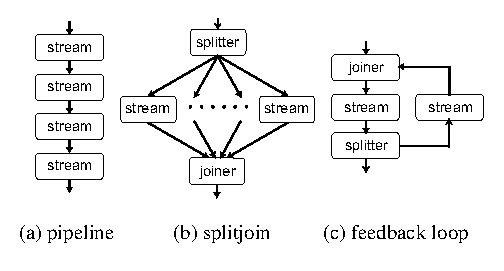
\includegraphics[scale=1, angle=0]{./constructs-eg.eps}
%}
% \vspace{-6pt}
% \nocaptionrule
 \caption{Hierarchical streams in StreamIt.}
 \label{fig:containers}
\end{center}
\end{figure}

\SubSection{Hierarchical Streams}
In StreamIt, the application developer focuses on the hierarchical
assembly of the stream graph and its communication topology, rather
than on the  explicit management of the data buffers between filters.
StreamIt provides three hierarchical structures for composing filters
into larger stream graphs (see Figure~\ref{fig:containers}).

\paragraph{Pipeline.}
The {\it pipeline} stream construct composes streams in sequence, with
the output of one connected to the input of the next.  An example of a
pipeline appears in Figure~\ref{fig:decoder-pipeline}. A pipeline is a
single input to single output stream. The decoding pipeline in the
figure consists of three streams. The first is a filter which zig-zag
unorders the input stream, and prepares the data for the inverse
quantization and DCT. The output of the filter is consumed by a stream
named {\tt IQ} which is a pipeline itself (not shown). This example
illustrates the hierarchical nature of stream composition in
StreamIt. The {\tt IQ} pipeline performs the inverse quantization, and
produces an output stream that is in turn consumed by another stream
which performs the inverse DCT. As in the case of a filter, pipelines
are also parameterizable.

\begin{figure*}[t]
  \begin{scriptsize}
    \begin{verbatim}
	int->int pipeline Decode()
	{ 
	  int Order[64] = {...};     // initialized as shown earlier
	  add ZigZagScan(64, Order);
	  add IQ();                  // inverse quantization
	  add IDCT(8, 8);            // inverse DCT (8x8 matrix)
	}
    \end{verbatim}
  \end{scriptsize}
  % \vspace{-3pt}
  \caption{Example MPEG decoder pipeline.}
  \label{fig:decoder-pipeline}
\end{figure*}

The {\tt add} keyword in StreamIt constructs the specified stream
using the input parameters. The {\tt add} statement may only appear in
non-filter streams.  In essence, filters are the leaves in the
hierarchical construction, and composite nodes in the stream graph
define the encapsulating containers. This allows for modular design
and development of large applications, thereby  promoting
collaboration, increasing code reuse, and simplifying debugging.

\paragraph{Split-Join.}
The {\it splitjoin} stream construct distributes data to a set of
parallel streams, which are then joined together in a roundrobin
fashion. In a splitjoin, the {\it splitter} performs the data
scattering, and the {\it joiner} performs the gathering. A splitter is
a specialized filter with a single input and multiple output
channels. On  every execution step, it can distribute its output to
any one of its children in either a {\it duplicate} or a {\it
roundrobin} manner. For the former, incoming data are replicated to
every sibling connected to the splitter. For the latter, data are
scattered in a roundrobin manner, with each item sent to exactly one
child stream, in order. The splitter type and the weights for
distributing data to child streams are declared as part of the syntax
(e.g., \texttt{split duplicate} or \texttt{split
roundrobin($w_1,\ldots,w_n$)}). The splitter counterpart is the
joiner. It is a specialized filter with  multiple input channels but
only one output channel. The joiner gathers data from its predecessors
in a roundrobin manner (declared as part of the syntax) to produce a
single output stream.

\begin{figure*}[t]
  \begin{scriptsize}
    \begin{verbatim}
	// N = macroblock size + motion vector data size;
	// W = picture width (resolution in pixels);
	// H = picture width (resolution in pixels);

	int->int splitjoin YCrCbDecoding(int N, int W, int H)
	{
	  // 4:2:0 chroma format
	  split roundrobin(4*N, 1*N, 1*N);

	  add LuminanceChannel  (W, H);
	  add ChrominanceChannel(W, H);
	  add ChrominanceChannel(W, H);

	  join roundrobin(1, 1, 1);  
	}
    \end{verbatim}
  \end{scriptsize}
  % \vspace{-3pt}
  \caption{Example MPEG decoder splitjoin.}
  \label{fig:decoder-sj}
\end{figure*}

The splitjoin stream is a convenient and natural way to represent
parallel computation. For example, when the decoder performs the
luminance and chrominance channel processing, the computation can
occur in parallel. In StreamIt, this is expressed as shown in
Figure~\ref{fig:decoder-sj}. The input stream contains the
macroblock data along with the parsed motion vectors. The data is
partitioned and passed to one of three decoding channels, with $4N$
items assigned to the first stream, $N$ items to the second, and $N$
items to the third. The three streams reconstruct the original
pictures with respect to the different color channels, and their
output is combined by the joiner to produce the final decoded picture.

\paragraph{Feedback Loop.}
StreamIt also provides a {\it feedback loop} construct for introducing
cycles in the graph. This stream construct is not used in the decoder,
but may be used in the MPEG encoder.

\paragraph{XXX: need to introduce messaging and talk about it.}
  \begin{figure*}[t]
  \centerline{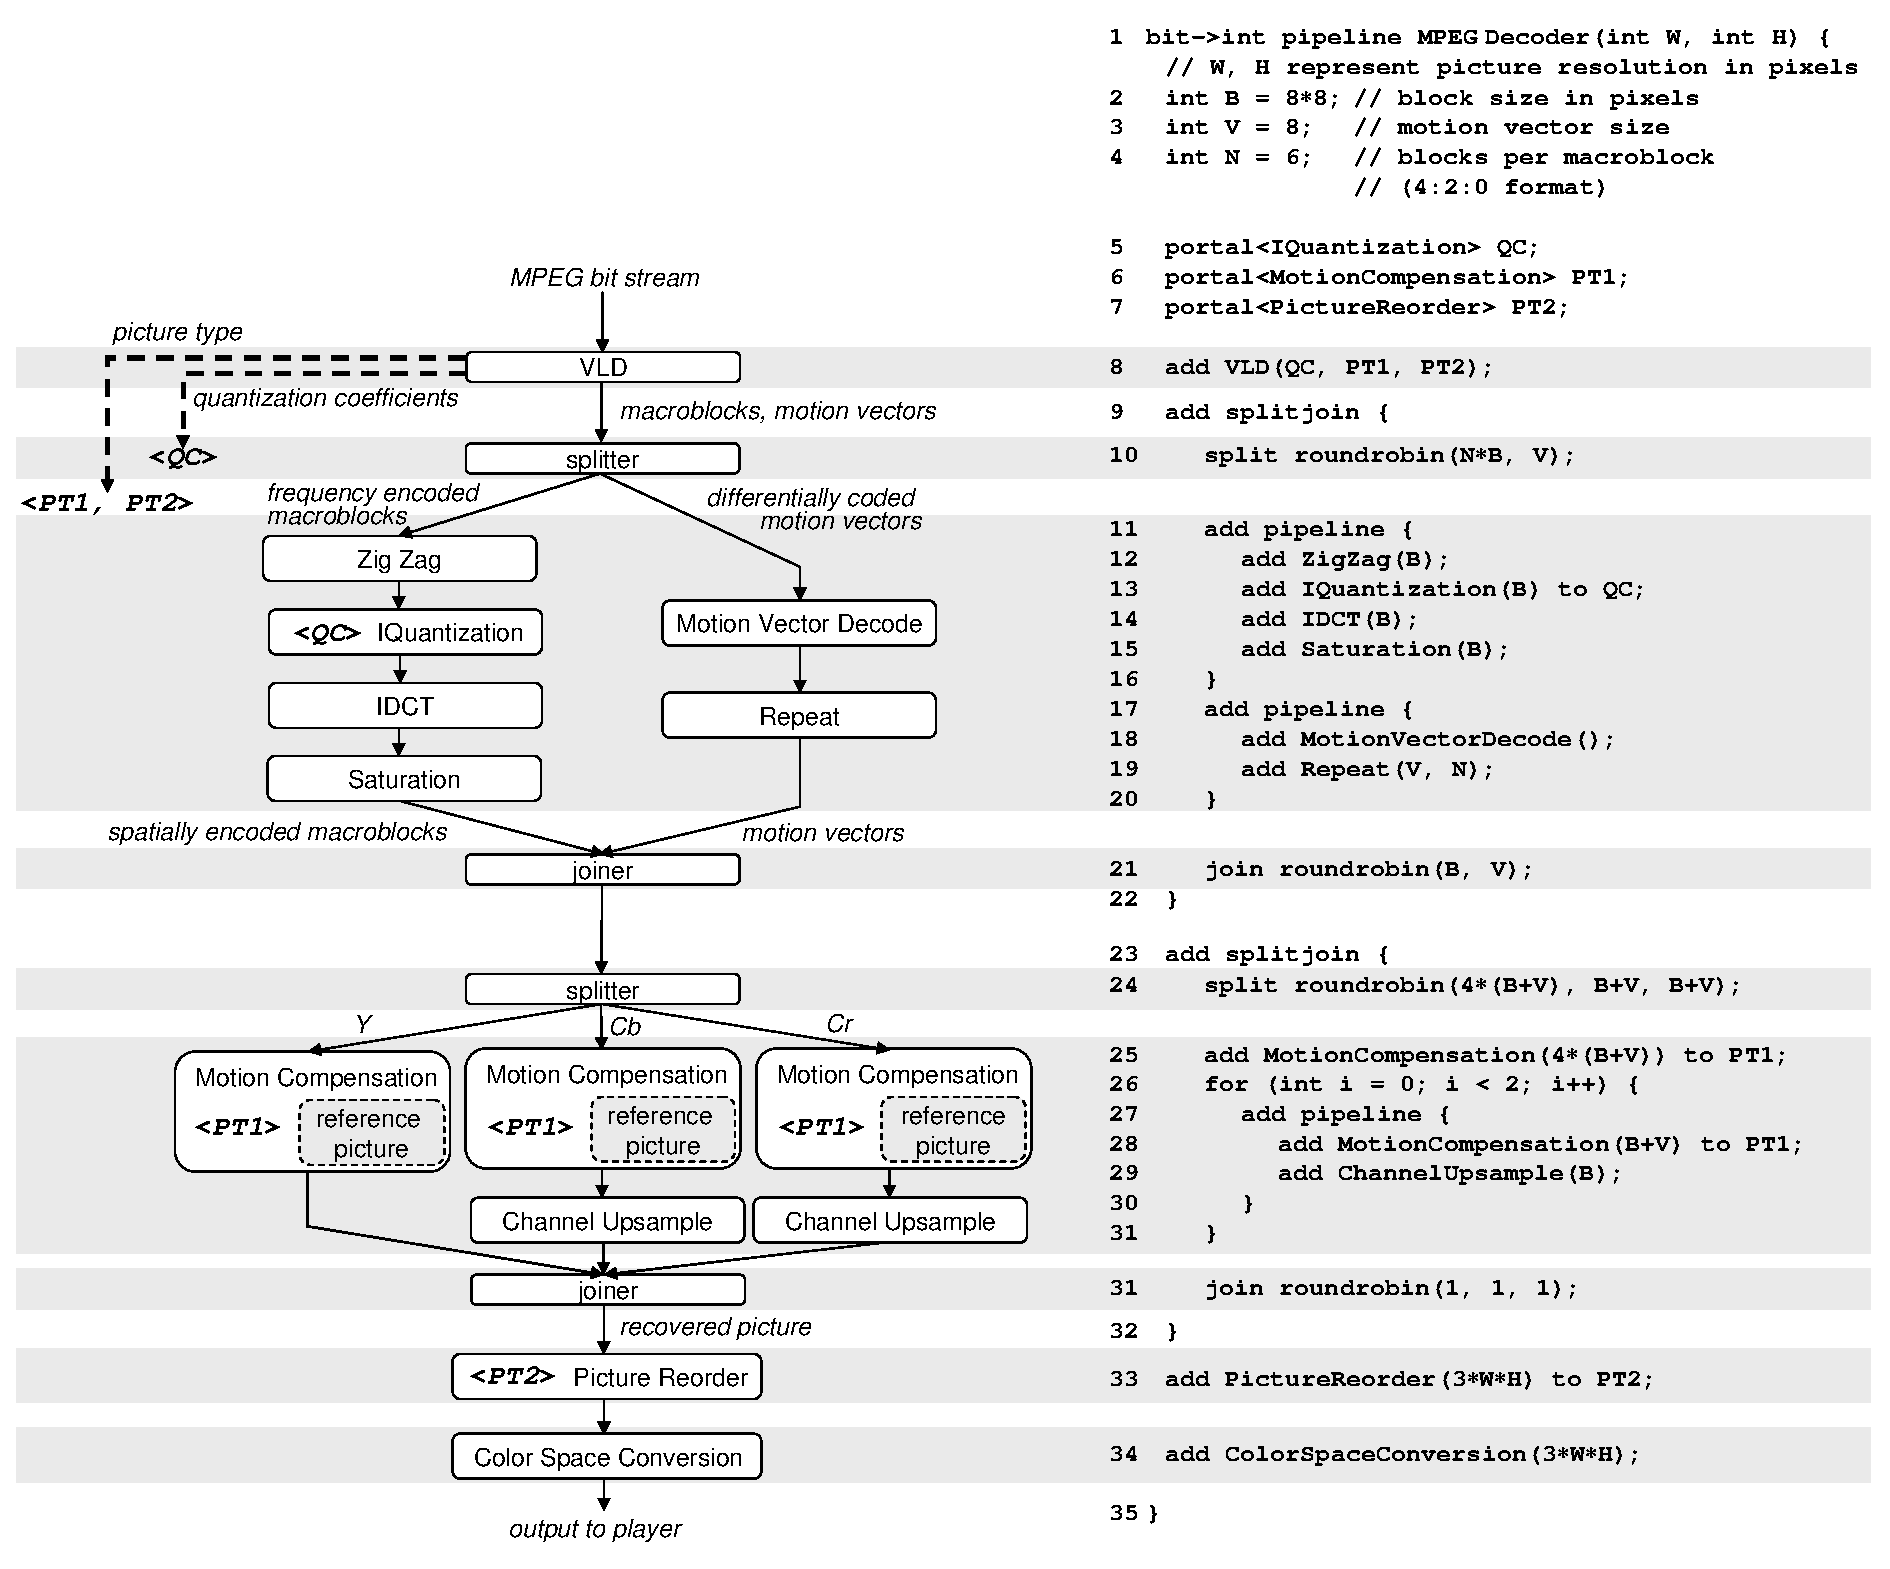
\epsfig{file=decoder_with_code.eps,width=5in}}
  \caption{MPEG-2 decoder block diagram and corresponding StreamIt code.}
  \label{fig:dec-with-code}
\end{figure*}

\Section{MPEG Decoder in StreamIt}

The MPEG decoder pipeline is shown in
Figure~\ref{fig:dec-with-code}. The stream graph is shown on the left,
alongside the StreamIt code on the right. It is worthy to note that
there is a high correlation between the stream block level diagram and
the StreamIt syntax describing the pipeline.

The decoder accepts a compressed bit stream as input, and produces the
decoded video stream as output. The computation is encapsulated in
three main components: the parser (line 8), the block and motion vector
decoder (lines 9-22), and the motion compensator (lines 23-34).

The parser is responsible for parsing the MPEG-2 bit stream and
performing Huffman and variable run-length decoding (VLD). The output
of the VLD is an interleaved stream of quantized macroblocks encoded
in the frequency-domain, and offset-encoded motion vectors. The VLD
outputs $\texttt{N}\times\texttt{B}$ data elements for each
macroblock, followed by \texttt{V} data elements that encode its
motion vector. The actual value of \texttt{N} depends on the chroma
format. In a 4:2:0 chroma format regime, $\texttt{N}=6$ since each
macroblock consists of four 8x8 subpixel blocks in the luminance channel,
and two 8x8 subpixel blocks in each of the two chrominance
channels. Therefore, the VLD outputs a total of six 8x8 blocks,
or 384 subpixels per macroblock.

The VLD output is segregated into two homogeneous streams by a
round robin splitter (line 7). The first stream undergoes inverse
transformations (lines 8-13), while the second is decoded to produce
absolute motion vectors (line 14). As is evident from the computation
graph, the two streams are decoded in parallel, and then merged (line
15) prior to the motion compensation stage of the pipeline.

The inverse transformations map each 8x8 block from the frequency
domain back to the spatially encoded domain. Each block is reordered
(line 9), and then inversely quantized (line 10). This is followed by
an inverse DCT and a bounded saturation filter (lines 11-12). The set
of transformations is grouped into a pipeline whose input
and output types are automatically inferred by the compiler. Each of
the filters in this pipeline operate on 8x8 blocks. The code that is
shown does not take advantage of data level parallelism between
blocks. It is rather straightforward however to expose this
parallelism if it is desirable. For example, in this case a splitjoin
can replicate the inverse transformation pipeline $N$ times:
\begin{center}
\begin{verbatim}
add splitjoin {
   split roundrobin(B);
   for (int i = 0; i < N; i++) 
      // add pipeline
   join roundrobin(B);
}
\end{verbatim}
\end{center}
A stream-aware compiler can also automatically adjust the execution
granularity as necessary~\cite{gordo-asplos}.  Data-parallel streams
can be easily identified as those that are stateless (i.e., do not
carry mutable state from one iteration to the next).

The third stage of the decoding pipeline performs the motion
compensation (lines 17-27) to recover predictively coded
macroblocks. The motion compensation filter uses the motion vectors to
find a corresponding macroblock in a previously decoded reference
picture. The reference macroblock is added to the current macroblock
to recover the original picture data. If the current macroblock is
part of an I or P picture, then the decoder stores it for use as a
future reference picture.

In the compensation stage, there are three parallel streams. 
The first handles the luminance color channel (Y), and the
other two handle the chrominance channels (Cb and Cr). The round robin
splitter (line 18) distributes the macroblocks according to the chroma
format. Since the luminance channel is not down sampled during the
encoding process, the splitter dispatches four 8x8 blocks at a time to
the Y motion compensator. The chrominance channels are typically down
sampled by a factor of 4, and hence one 8x8 block is streamed to each
of the Cb and Cr pipelines, which up sample (line 23) the results of
the motion compensator to generate the full 16x16 macroblock.  The
joiner (line 26) assembles the pictures from each of the color
channels, one pixel at a time. The output is then readied for display
(lines 28 and 29) by organizing the pictures in accord with their
temporal order, and performing color space conversion to the RGB (red,
green, blue) color model. Note that these two filters each consume
$3\times\texttt{W}\times\texttt{H}$ subpixels per picture. This is three
times the pixel resolution of the decoded image since there is one
pixel generated from each of the three channel decoders. The output of
the decoder is $\texttt{W}\times\texttt{H}$ pixels in the end.

The MPEG-2 decoder in StreamIt is a fully portable implementation in
that the application is not architecture dependent. The implementation
naturally exposes the pipeline parallelism that exists throughout the
decoder, as well as the data level parallelism inherent to the inverse
transformations and motion compensation.

The implementation was carried out by one student programmer with no
prior understanding of MPEG. The development spanned eight weeks from
specification~\cite{MPEG2} to the first fully functional MPEG
decoder. The StreamIt code is nearly 3,165 lines of code with 48
static streams. The bit stream parser is the largest single filter,
consisting of 775 lines of code. The 48 static streams are compiled to
2,150 filters for a picture resolution of 352x240. By way of
comparison, the reference C implementation~\cite{reference-mpeg-c} is
6,835 lines of code. A line count comparison is not an accurate
measure of programmability, and our StreamIt decoder 
implements only a subset of several stream types supported by MPEG.
Our decoder does provide full support for the range of different 
compression techniques used within MPEG, but supports only a subset 
of the possible display modes (i.e. interlaced versus progressive output).
However, these alternate display formats represent minor conceptual
changes and should therefore affect small portions of the StreamIt code. 
This is demonstrated in Section~\ref{section:chroma} with an example of
support for multiple chrominance formats. 

The reference C implementation intermingles parsing, decoding, and
motion compensation, making it difficult to clearly follow the code,
and hindering a better comparison. The C code also relies on global
variables to communicate values, such as quantization coefficients,
from the parser to the relevant code regions. In StreamIt, such
communication is relegated to teleport messaging (lines 5, 10, 22, and
28, and illustrated with dotted lines in
Figure~\ref{fig:dec-with-code}). For instance, the parser (VLD)
generates a message whenever the picture or macroblock type
changes. The motion compensation filter receives this information via
its dedicated portal (line 22), determines how to process the current
picture, and decides whether it needs to store it for future
reference. The picture reordering filter receives a similar message
(via portal on line 28), and uses the information to determine the
correct temporal order of pictures. The inverse transformation
pipeline listens to its portal (line 10) to determine the algebraic
manipulation required to perform the inverse quantization of the input
macroblock. Teleport messaging proves as a natural mechanism because
the macroblock type and picture type information changes infrequently
and irregularly, compared to the regular flow of data in the
application. Moreover, by exposing the flow of messages to the
compiler, the application can be reordered or parallelized without a
heroic dependence analysis.

In StreamIt, all of the processing is encapsulated hierarchically into
single-input, single-output streams with well-defined modular
interfaces. This property facilitates development and boosts
programmer productivity, as components can be debugged and verified as
standalone components. The modularity also promotes reuse. For
example, the zig-zag descrambler, inverse quantizer, and inverse DCT
components may be used as is to implement a JPEG decoder.

Another noteworthy aspect of the StreamIt implementation is its
malleability. We illustrate this by outlining how the decoder
implementation, originally designed to deal with a 4:2:0 chroma
sampling rate is modified for a 4:2:2 sampling rate. MPEG-2 streams
are typically encoded using the former, which achieves a 50\%
reduction in the number of bits required to represent a
video. However, better quality is possible with higher sampling rates
since more color information is retained from the original picture. In
this sequel, we show that the migration path to support multiple
chroma formats is trivial.

\SubSection{Video Sampling Rate}

Macroblocks specify colors using a luminance channel to represent
saturation (color intensity), and two chrominance channels to
represent hue. The human eye is more sensitive to changes in
saturation than changes in hue, so the chrominance channels are
frequently compressed by downsampling the chrominance data within a
macroblock. The type of chrominance downsampling an MPEG-2 encoder
uses is its {\it chrominance format}. The most common chrominance
format is 4:2:0, which uses a single block for each of the chrominance
channels, downsampling each of the two channels from 16x16 to 8x8.
The other chrominance format with downsampling is 4:2:2, which uses
two blocks for each chrominance channel, downsampling each of the
channels from 16x16 to 8x16. The possible chrominance formats are
shown in Figure~\ref{fig:chroma-format}.

To support the 4:2:2 chrominance format in our StreamIt decoder, we
modified 31 lines and added 20 new lines. Of the 31 modified lines, 23
were trivial modifications to pass a variable representing the
chrominance format as a stream parameter. The greatest substantial
change was to the decoding splitjoin previously illustrated in
Figure~\ref{fig:decoding-sj}. The stream is reconfigured such that it
can properly deal with the interleaving of chrominance data when the
sampling rate is increased. The more general splitjoin is shown in
Figure~\ref{fig:chroma-stream}.

%% TODO: add figure showing pattern for 4:2:0 and 4:2:2 and expand on
%% description above
\begin{figure*}[t]
  \begin{scriptsize}
    \begin{verbatim}
    int->int splitjoin(int chromaFormat) {
      int xUpSample, yUpSample;

      if (chromaFormat == 420) { // 4:2:0 chroma format
        split roundrobin(4*N, 2*N);
	  xUpSample = yUpSample = 2;
      } else {                   // 4:2:2 chroma format
        split roundrobin(4*N, 4*N);
	  xUpSample = 2;
	  yUpSample = 0;
      }

      add LuminanceChannel(W, H, 0, 0, chromaFormat);

      add int->int splitjoin {
        split roundrobin(N, N);
        add ChrominanceChannel(W, H, xUpsample, yUpSample, chromaFormat);
        add ChrominanceChannel(W, H, xUpsample, yupsample, chromaFormat);
        join roundrobin(1, 1);
      }

      join roundrobin(1, 2);
  }
  \end{verbatim}
  \end{scriptsize}
  % \vspace{-3pt}
  \caption{Decoding stream to handle 4:2:0 and 4:2:2 chroma formats.}
  \label{fig:chroma-stream}
\end{figure*}


%% \SubSection{Motion Compensation}

% Commented out this section since this information is incorporated into
% the decoder implementation section. - Matt 1/25/06
% An MPEG decoder accepts a bitstream as input and performs Huffman and
% variable run-length decoding (VLD).  This process results in a set of
% quantized, frequency-domain macroblocks and corresponding motion
% vectors.  The decoder inversely quantizes (IQ) the macroblocks and then
% performs an inverse DCT (IDCT) to convert the macroblocks to the
% spatial domain.  For predictively coded macroblocks (e.g., P and B
% pictures), the decoder performs motion compensation (MC) using the
% input motion vectors to find a corresponding macroblock in a
% previously decoded, stored reference picture. This reference
% macroblock is added to the current macroblock to recover the original
% picture data. If the current macroblock is part of an I or P picture,
% then the decoder stores it for future reference.
% Figure~\ref{fig:dec_block} illustrates the decode sequence.

%\begin{figure}[htbp]
%\centerline{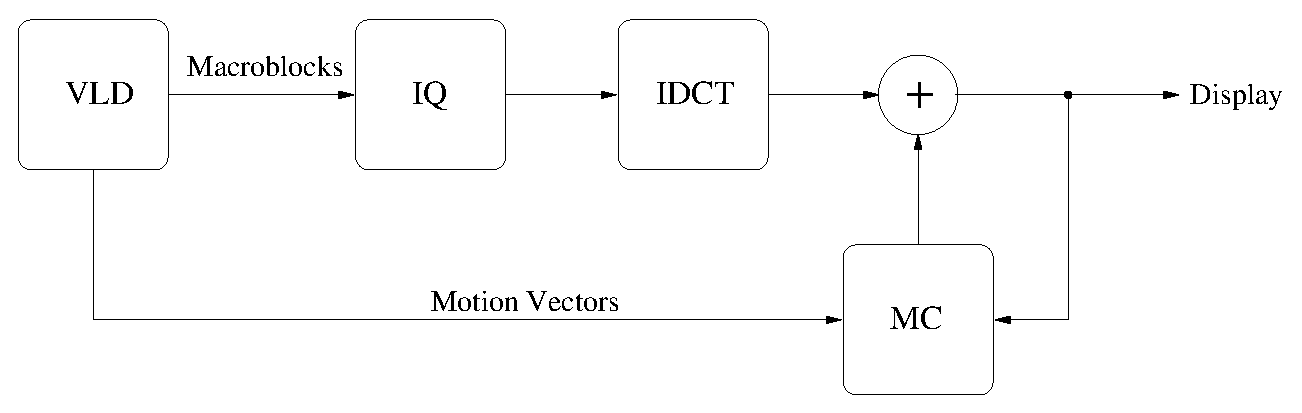
\epsfig{file=dec_block.eps,width=5in}}
%\caption{Block diagram of MPEG-2 decode.}
%\label{fig:dec_block}
%\end{figure}

%% A simple strategy for parallelizing the MPEG-2 decoding can exploit
%% the data parallelism among macroblocks. Using this scheme, the Huffman
%% and run-length decoding is inherently serial, as macroblock boundaries
%% can only be discovered by performing the decode operation.  Once this
%% decode is complete, a parallel implementation can distribute
%% macroblocks to independent streams (using a splitjoin). Each stream
%% performs the inverse quantization, inverse discrete cosine transform,
%% and motion compensation. Furthermore, each stream locally stores
%% reference macroblocks for future motion compensation. Using this
%% strategy, the streams can execute independently with one exception.

%% % TODO: This is the figure showing the macroblock parallelism
%% % I'm not sure where it goes. - Matt
%% \begin{figure*}[t]
%% \vspace{-12pt}
%% %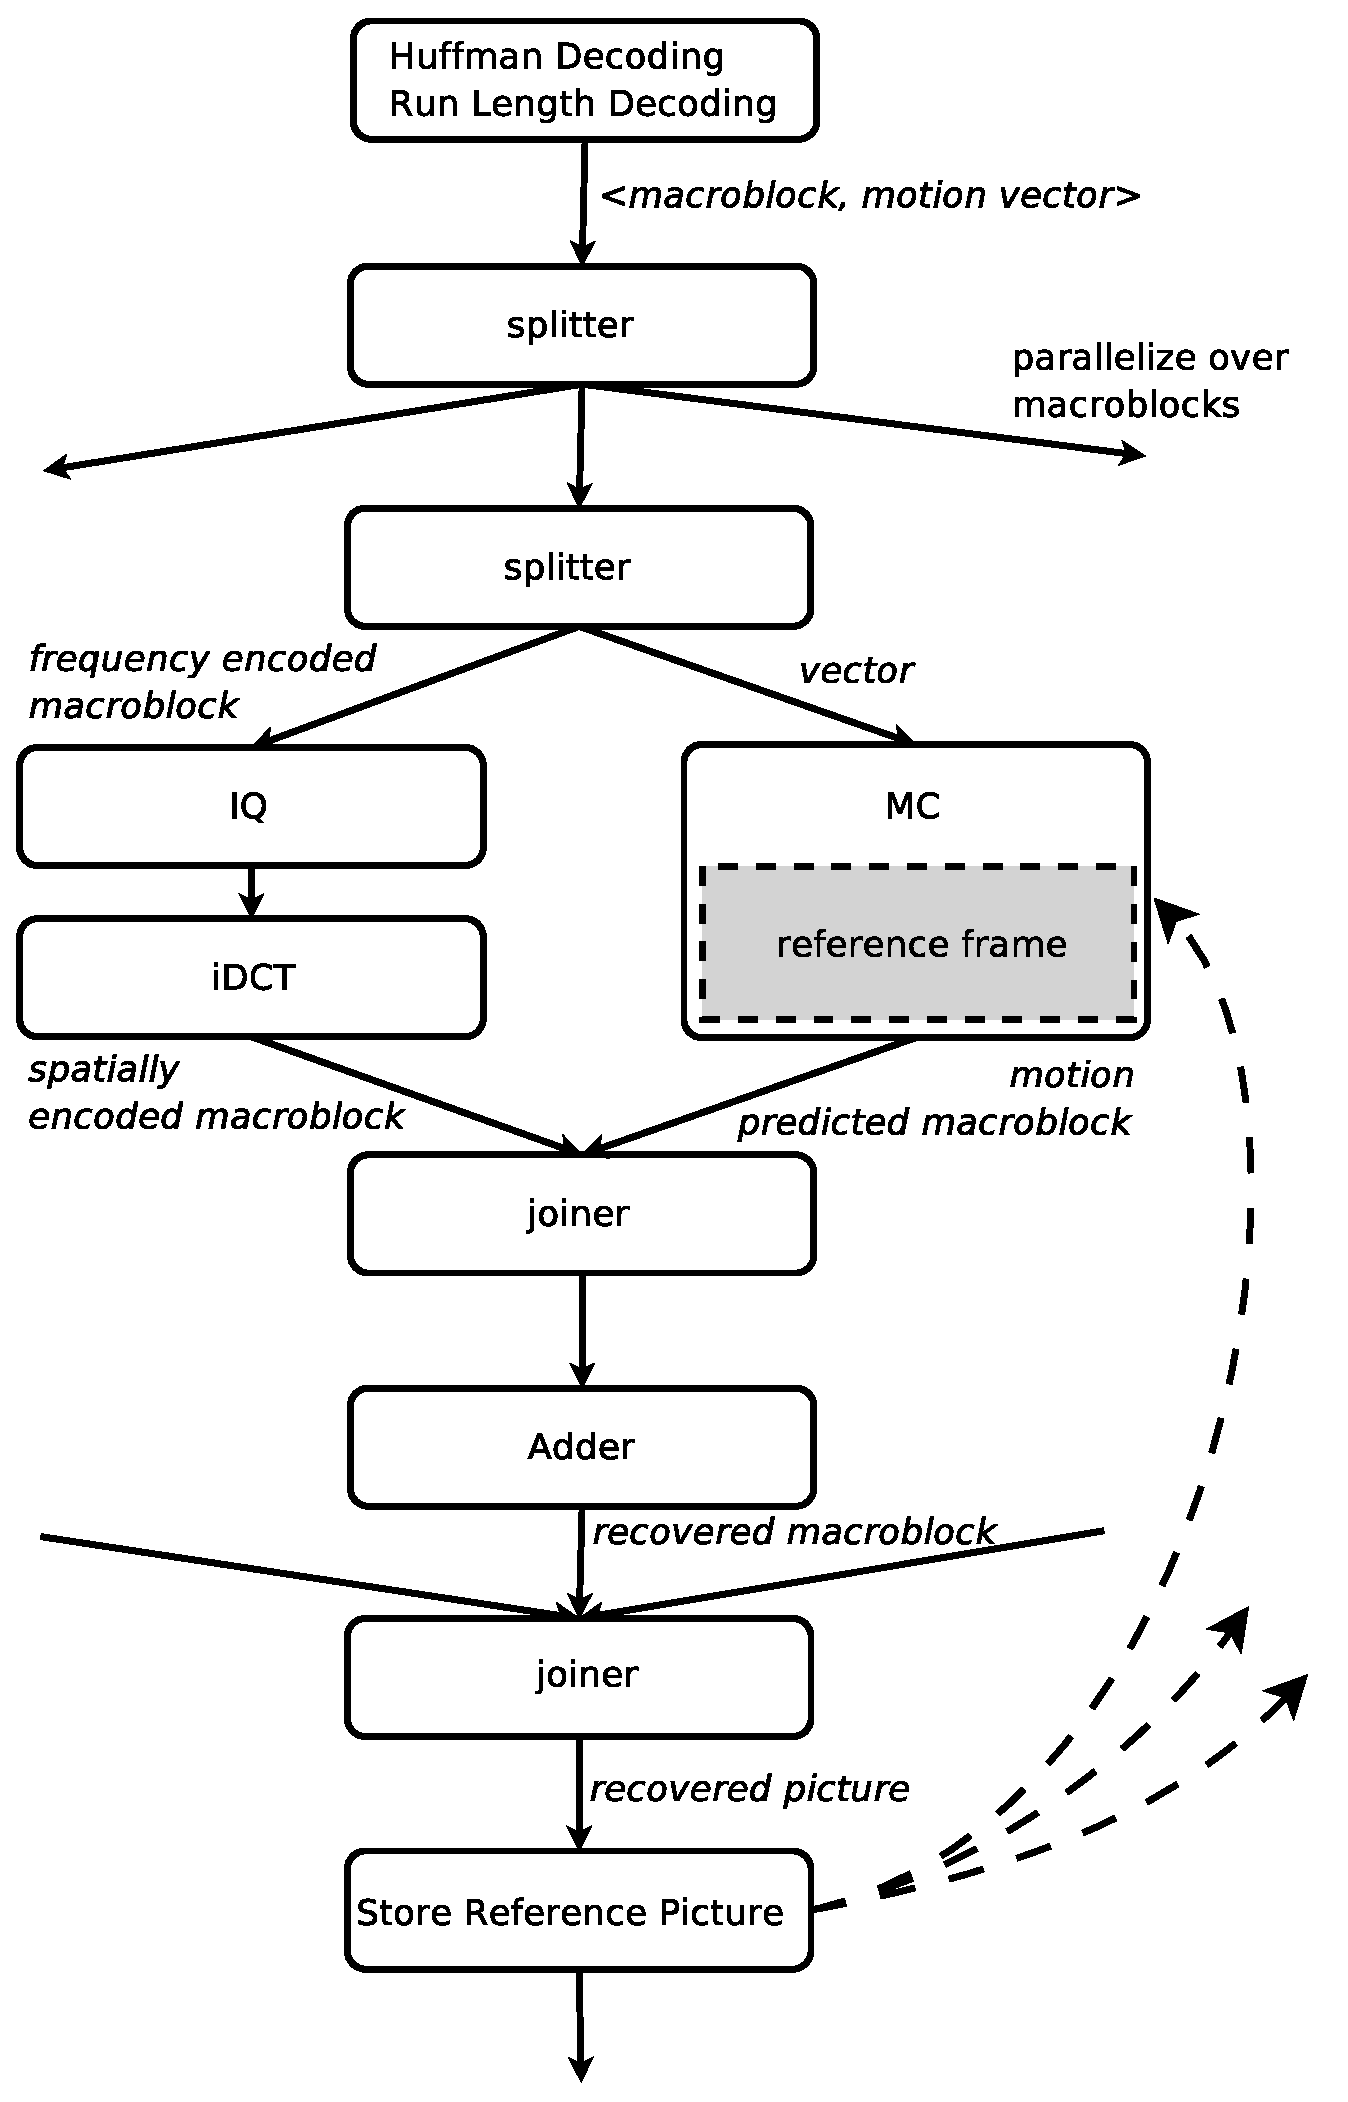
\epsfig{file=decoder_macroblock_parallelism.eps, width=3in}
%% %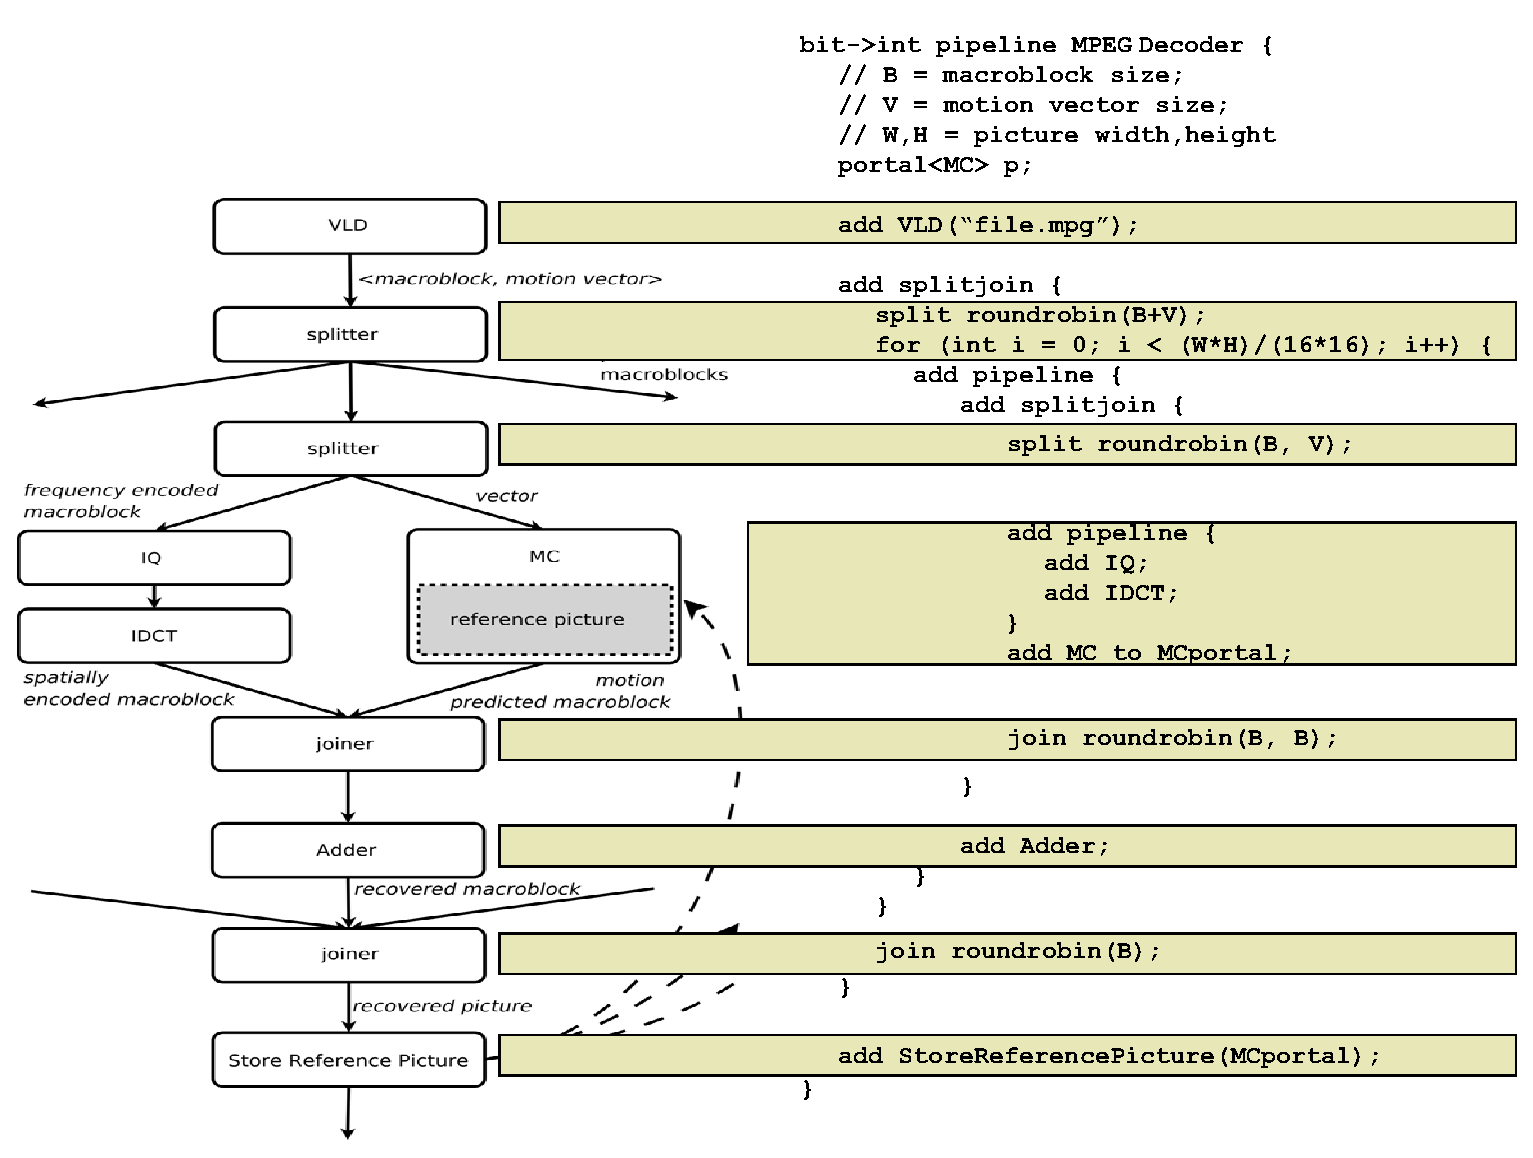
\epsfig{file=decoder-parallel.eps, width=\textwidth}
%% 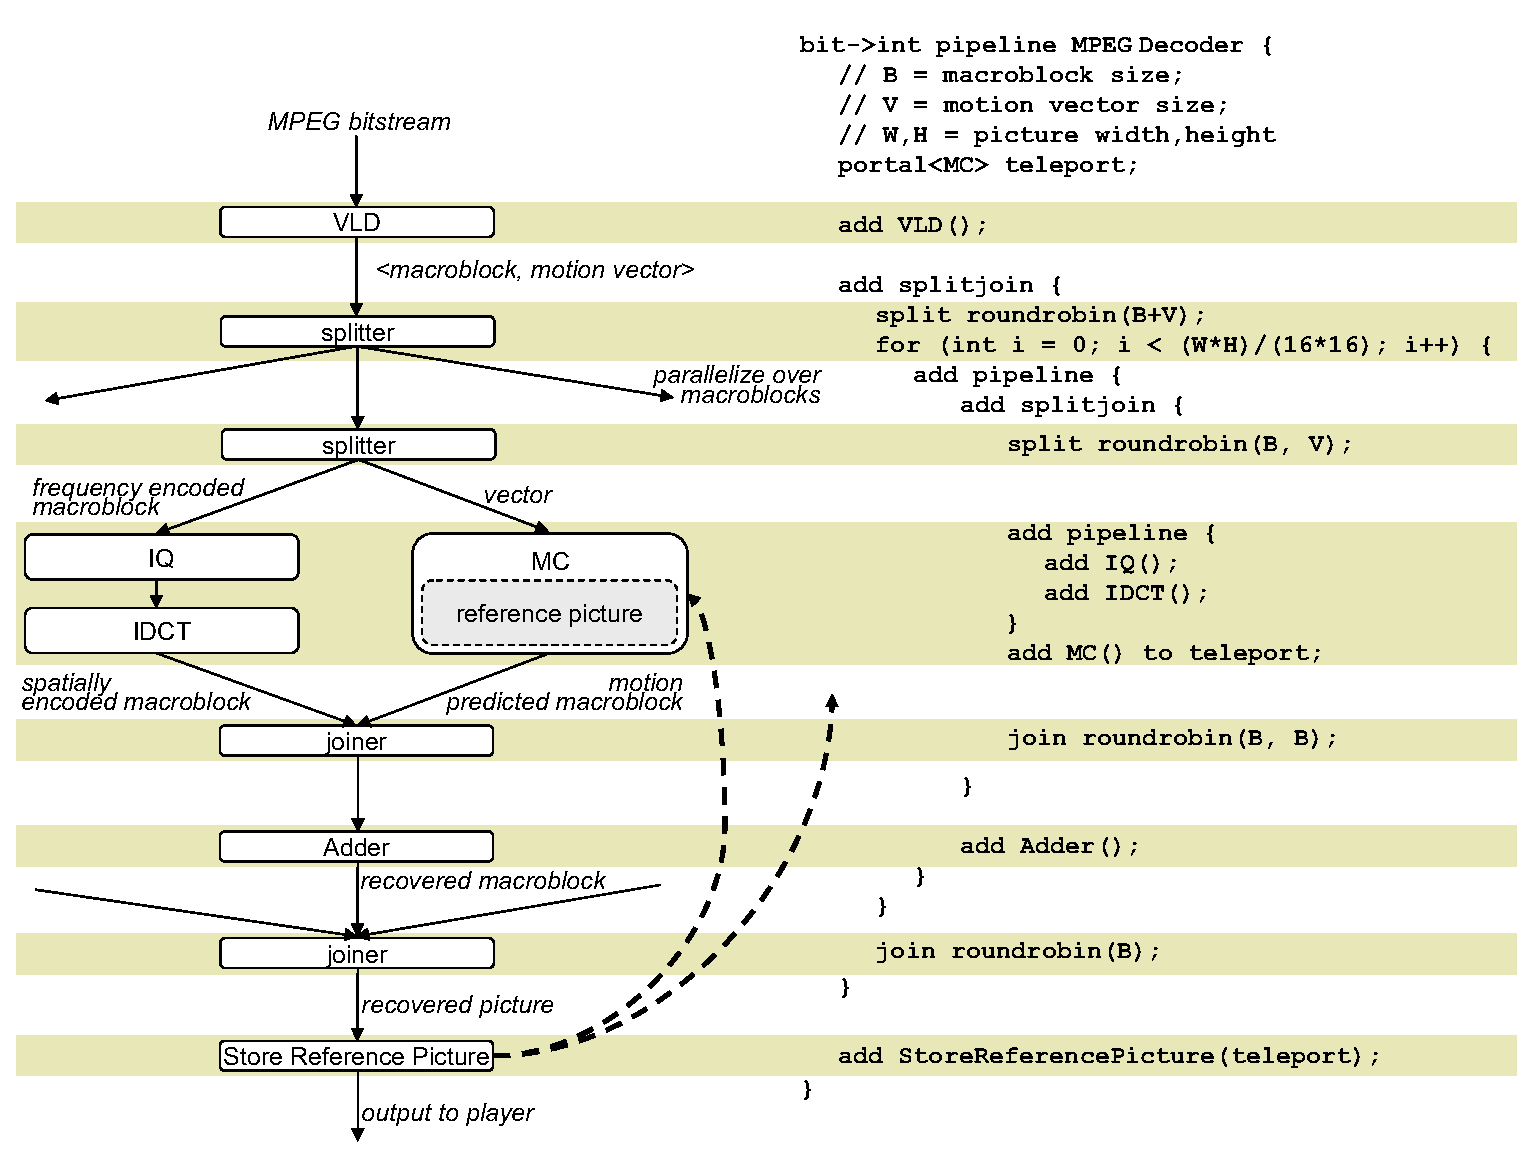
\epsfig{file=decoderpipeline.eps, width=\textwidth}
%% % TODO: Change Matt's 2 am caption.
%% \caption{MPEG-2 decoder exploiting macroblock-level parallelism.}
%% \label{decoder_macroblock_parallelism}
%% \vspace{-6pt}
%% \end{figure*}

%% This exception occurs when a stream is performing motion compensation
%% and the corresponding motion vector indicates a reference macroblock
%% stored in some other stream. In this case, inter-stream communication
%% is required to send the reference data to the requesting stream. This
%% situation is not uncommon, and is more prevalent for higher resolution
%% pictures. A simple scheme for handling this situation is for every
%% stream to broadcast its decoded macroblocks to all other streams. This
%% solution has the benefit of being conceptually easy to understand and
%% implement. StreamIt allows programmers to naturally expose such
%% parallelism.
%% A StreamIt pipeline that operates at macroblock
%% granularity is shown in Figure~\ref{decoder_macroblock_parallelism}. It is
%% worthy to note that there is a high correlation between the stream
%% graph, and the StreamIt syntax describing the pipeline.

%% The implementation can be made more fine grained by exposing the
%% intra-macroblock parallelism. For example, the IQuantization-IDCT
%% pipeline can operate at a block level, rather than at a macroblock
%% granularity. This is easily achieved by encapsulating the  pipeline
%% within a splitjoin to scatter the blocks, operate, and gather the
%% results to recover the parent macroblock.

%% There are many implementation strategies for the decoder, each with
%% varying degrees of exposed parallelism. Of the greatest advantage of
%% the StreamIt implementation is its malleability. The stream graph is
%% easily reconfigured to operate at picture-level granularity (exposing
%% parallelism between chroma channels), macroblock level (exposing even
%% more data-level parallelism), or even at block level (exposing the
%% greatest amount of data-level parallelism).
  \SubSection{Video Sampling Rate}

Macroblocks specify colors using a luminance channel to represent
saturation (color intensity), and two chrominance channels to
represent hue. The human eye is more sensitive to changes in
saturation than changes in hue, so the chrominance channels are
frequently compressed by downsampling the chrominance data within a
macroblock. The type of chrominance downsampling an MPEG-2 encoder
uses is its {\it chrominance format}. The most common chrominance
format is 4:2:0, which uses a single block for each of the chrominance
channels, downsampling each of the two channels from 16x16 to 8x8.
The other chrominance format with downsampling is 4:2:2, which uses
two blocks for each chrominance channel, downsampling each of the
channels from 16x16 to 8x16. The possible chrominance formats are
shown in Figure~\ref{fig:chroma-format}.

To support the 4:2:2 chrominance format in our StreamIt decoder, we
modified 31 lines and added 20 new lines. Of the 31 modified lines, 23
were trivial modifications to pass a variable representing the
chrominance format as a stream parameter. The greatest substantial
change was to the decoding splitjoin previously illustrated in
Figure~\ref{fig:decoding-sj}. The stream is reconfigured such that it
can properly deal with the interleaving of chrominance data when the
sampling rate is increased. The more general splitjoin is shown in
Figure~\ref{fig:chroma-stream}.

%% TODO: add figure showing pattern for 4:2:0 and 4:2:2 and expand on
%% description above
\begin{figure*}[t]
  \begin{scriptsize}
    \begin{verbatim}
    int->int splitjoin(int chromaFormat) {
      int xUpSample, yUpSample;

      if (chromaFormat == 420) { // 4:2:0 chroma format
        split roundrobin(4*N, 2*N);
	  xUpSample = yUpSample = 2;
      } else {                   // 4:2:2 chroma format
        split roundrobin(4*N, 4*N);
	  xUpSample = 2;
	  yUpSample = 0;
      }

      add LuminanceChannel(W, H, 0, 0, chromaFormat);

      add int->int splitjoin {
        split roundrobin(N, N);
        add ChrominanceChannel(W, H, xUpsample, yUpSample, chromaFormat);
        add ChrominanceChannel(W, H, xUpsample, yupsample, chromaFormat);
        join roundrobin(1, 1);
      }

      join roundrobin(1, 2);
  }
  \end{verbatim}
  \end{scriptsize}
  % \vspace{-3pt}
  \caption{Decoding stream to handle 4:2:0 and 4:2:2 chroma formats.}
  \label{fig:chroma-stream}
\end{figure*}

  %\section{The StreamIt Compiler}
\label{sec:compiler}


\begin{table*}[t]
\begin{center}
\scriptsize
\begin{tabular}{|l|l|} \hline
{\bf Phase} & {\bf Function} \\
\hline \hline
KOPI Front-end & Parses syntax into a Java-like abstract syntax tree. \\
\hline
SIR Conversion & Converts the AST to the StreamIt IR (SIR). \\
\hline
Graph Expansion & Expands all parameterized structures in the stream graph. \\
\hline
Scheduling & Calculates initialization and steady-state execution orderings for filter firings. \\
\hline
Partitioning & Performs fission and fusion transformations for load balancing. \\
\hline
Layout & Determines minimum-cost placement of filters on grid of Raw tiles. \\
\hline
Communication Scheduling & Orchestrates fine-grained communication between tiles via simulation of the stream graph. \\
\hline
Code generation & Generates code for the tile and switch processors. \\
\hline
\end{tabular}
\caption{\protect\small Phases of the StreamIt compiler.
\label{tab:phases}}
\end{center}
\end{table*}

The phases of the StreamIt compiler are described in
Table~\ref{tab:phases}.  The details of each stage can be found in
~\cite{streamit-asplos}.  The following subsections provide an
overview on the phases of the StreamIt compiler and the changes made
to the corresponding phases to implement the iteration keyword.

\subsection{StreamIt Compiler Overview}
\label{sec:compiler-overview}

The front end is built on top of KOPI, an open-source compiler 
infrastructure for Java~\cite{kopi}.  We translate the KOPI syntax 
tree into the StreamIt IR (SIR) that encapsulates the hierarchical 
stream graph.  The graph is then expanded for structures that
are parametrized.  Constants are propagated through the program
and the graph is expanded into a static structure.

We can calculate an execution schedule for the nodes of the stream 
graph.  The schedule indicates a multiplicity for each filter in the
stream graph, which determines how often the work function should be
invoked.  The schedule is periodic, meaning its
execution must preserve the number of live items on each channel in
the graph.  Accordingly, there is a {\it steady-state} schedule that is 
periodic which maintains this invariant.  Peeking filters, however, 
introduce another layer of complication.
A filter with {\it peek $>$ pop} leaves {\it peek - pop} items on the
input channel after every firing.  If the periodic schedule contains
these extra items, every firing would leave leftover items
in the channel.  Accordingly, peeking filters require a separate,
non-periodic {\it intialization} schedule.  

{\it Partitioning} is the process of dividing the stream program into
a set of balanced computation units.  Given a number $N$, representing
the maximum number of computation units that can be supported, the 
partitioning step transforms a stream graph into a set of at most $N$
load-balanced filters.  Each filter can be run on a separate processor.
The partitioning step uses a set of fusion, fission, and reordering 
transformations to achieve the desired granularity and load-balancing~\cite{streamit-asplos}.

The {\it layout} phase assigns nodes in the stream graph to the
computation nodes in the target architecture while minimizing the
communication and synchronization in the final layout.  The {\it
communication scheduling} phase maps the communication explicit
in the stream graph to the interconnect of the target.  The FIFO
abstraction of the stream channels is mapped to the limited resources
of the target.  Finally, {\it code generation} is performed using the
results of all previous phases.  
  %\Section{MPEG Encoder in StreamIt}
  \mysection{Related Work}
\label{sec:related}

This paper builds directly on the work done to analyze and optimize
linear components in StreamIt graphs \cite{Lamb}. We extend the
theoretical framework for linear analysis to state space analysis in
order to apply our optimizations to a wider class of applications.
Specifically, state space analysis applies to filters with persistent
state, and feedback loops can be combined into a single state space
representation; neither of these cases are handled by linear analysis.
The extension from linear analysis to state space analysis required a
fundamental change to the underlying representation, as well as a
complete reformulation of the rules for combination and expansion.
Moreover, this paper introduces novel optimizations of state removal
and minimal parameterization, both of which operate on the state space
representation.

Several other groups are researching methods for automated DSP
optimizations. SPIRAL \cite{Spiral} is a system developed to generate
libraries of DSP transforms. These libraries are designed for specific
architectures, and can be re-optimized when hardware is upgraded or
replaced. Other such libraries that have been designed include a
package for linear algebra manipulations by the ATLAS project
\cite{Atlas} and portable high-performance FFTs (Fast Fourier
Transforms) \cite{fftw}.

Aside from StreamIt, other programming languages have been designed
for streaming data. Synchronous languages which target embedded
applications include LUSTRE \cite{Lustre}, Esterel \cite{Esterel}, and
Signal \cite{Signal}. Other stream-based languages are Occam
\cite{Occam}, SISAL \cite{sisal}, and StreamC \cite{streamc}.  Some of
these languages are designed to exploit vector and parallel
processing. However, none of these languages have compilers that run
state space or linear analysis.

  %\section{Future Work}
\label{sec:future}

%% First, as the current transformation has the potential to increase the
%% size of the file, we plan to explore lightweight techniques for
%% re-compressing a data stream that is already partially compressed.
%% This should be straightforward in the case of Apple Animation; for
%% example, a run-length encoded unit can be extended without needing to
%% be rediscovered.

There remain rich areas for future work in computing on compressed
data.  First, the compressed processing technique can be applied far
beyond the current focus.  In its current form, the technique could be
evaluated on video operations such as thresholding, color depth
reduction, sepia toning, saturation adjustment, and color replacement.
With minor extensions (see Section~\ref{sec:extensions}), the
technique can support video operations such as cropping, padding,
histograms, image flipping, sharpening, and blurring.  The technique
may also have applications in an embedded setting, where it could
offer power savings---for example, in processing the RAW data format
within digital cameras.  It may even be possible to do sparse matrix
operations using the technique; in addition to compressing the
locations of the zero elements, LZ77 would also compress repetetive
patterns in the non-zero elements.

Research is also underway to apply a similar technique to lossy,
DCT-based compression formats.  The streaming model cf computation
also offers key advantages in this domain, as neighboring actors that
compute linear functions can be algebraically simplified at compile
time~\cite{aalamb}.  For example, a JPEG transcoder typically performs
an iDCT (during decompression), followed by the user's transformation,
followed by a DCT (during compression).  If the user's transformation
is also linear (e.g., color inversion) then all three stages can be
automatically collapsed, thereby eliminating the decompression and
re-compression steps.  Preliminary experiments in this direction
indicate speedups upwards 10x.  By extending the framework to multiple
compression formats, users will be able to write their transformations
once, in a high-level language, and rely on the compiler to map the
computations to each of the compresed domains.


  \section{Conclusion}

This paper shows that the inter-node dependences of a Cyclo-Static
Dataflow Graph can be cleanly represented as a System of Affine
Recurrence Equations.  In combination with Feautrier's array dataflow
analysis~\cite{Feautrier01} for deducing intra-node dependences, this
establishes the SARE as a unified analysis and optimization framework
for high-level DSP programming models.

We believe that the precise affine dependence framework provided by
the SARE representation will enable a powerful suite of node
optimizations in dataflow graphs.  The SARE is a robust and
well-established framework within the systolic and scientific
communities, with methods for graph parameterization, automatic
parallelization, and storage optimization.  We propose optimizations
such as decimation propagation and node fission that are first
applications of these techniques to the signal processing domain.

  
  \vspace{-2pt}
  \section*{Acknowledgements}
  \vspace{-7pt}
  We are very grateful to the entire StreamIt team for their hard work
  and insightful comments. Allyn Dimock, Michael Gordon, Janis
  Sermulins, and especially William Thies, contributed immensely to
  the StreamIt infrastructure to enable this paper. We also thank the
  anonymous reviewers for their helpful suggestions. The StreamIt
  project is supported by DARPA grants PCA-F29601-03-2-0065 and
  HPCA/PERCS-W0133890, and NSF awards CNS-0305453 and EIA-0071841.

%  \bibliographystyle{ipdps}
%  \bibliography{main}
  \vspace{-2pt}
\begin{thebibliography}{10}\setlength{\itemsep}{-1ex}\small
  \vspace{-7pt}
\bibitem{agrawal05cases}
S.~Agrawal, W.~Thies, and S.~Amarasinghe.
\newblock Optimizing stream programs using linear state space analysis.
\newblock In {\em {CASES}}, 2005.

\bibitem{ahmad01multiproc}
I.~Ahmad, S.~M. Akramullah, M.~L. Liou, and M.~Kafeel.
\newblock {A Scalable Off-line MPEG-2 Video Encoding Scheme using a
  Multiprocessor System}.
\newblock {\em {Parallel Computing}}, 27, 2001.

\bibitem{ahmad01compression}
I.~Ahmad, Y.~He, and M.~L. Liou.
\newblock {Video compression with parallel processing}.
\newblock {\em {Parallel Computing}}, 28, 2002.

\bibitem{ph}
S.~Aidtya, Arvind, L.~Augustsson, J.~Maessen, and R.~S. Nikhil.
\newblock {Semantics of pH: A parallel dialect of Haskell}.
\newblock In {\em Haskell Workshop}, 1995.

\bibitem{Lucid77}
E.~Ashcroft and W.~Wadge.
\newblock Lucid, a non procedural language with iteration.
\newblock {\em C. ACM}, 20(7), 1977.

\bibitem{assayad05mpeg4b}
I.~Assayad, P.~Gerner, S.~Yovine, and V.~Bertin.
\newblock {Modelling, Analysis and Parallel Implementation of an On-line Video
  Encoder}.
\newblock In {\em {1st Int. Conf. on Distributed Frameworks for Multimedia
  Applications}}, 2005.

\bibitem{Esterel}
G.~Berry and G.~Gonthier.
\newblock {The Esterel Synchronous Programming Language: Design, Semantics,
  Implementation}.
\newblock {\em Sci. of Comp. Programming}, 19(2), 1992.

\bibitem{brook04}
I.~Buck, T.~Foley, D.~Horn, J.~Sugerman, K.~Fatahalian, M.~Houston, and
  P.~Hanrahan.
\newblock {Brook for GPUs: Stream Computing on Graphics Hardware}.
\newblock In {\em SIGGRAPH}, 2004.

\bibitem{Lucid-Synchrone}
P.~Caspi and M.~Pouzet.
\newblock {Lucid Synchrone distribution}.
\newblock {\tt http://www-spi.lip6.fr/lucid-synchrone/}.

\bibitem{spidle03}
C.~Consel, H.~Hamdi, L.~R�veill�re, L.~Singaravelu, H.~Yu, and C.~Pu.
\newblock {Spidle: A DSL Approach to Specifying Streaming Application}.
\newblock In {\em {2nd Int. Conf. on Generative Prog. and Component
  Engineering}}, 2003.

\bibitem{Occam}
I.~Corporation.
\newblock {\em Occam 2 Reference Manual}.
\newblock Prentice Hall, 1988.

\bibitem{kock02jpeg}
E.~de~Kock.
\newblock {Multiprocessor Mapping of Process Networks: A JPEG Decoding Case
  Study}.
\newblock In {\em {15th Int. Symp. on System Synthesis}}, 2002.

\bibitem{kock00yapi}
E.~de~Kock, G.~Essink, W.~Smits, P.~van~der Wolf, J.~Brunel, W.~Kruijtzer,
  P.~Lieverse, and K.~Vissers.
\newblock {YAPI: Application Modeling for Signal Processing Systems}.
\newblock In {\em {Conf. on Design Automation}}, 2000.

\bibitem{dwivedi01exploring}
B.~K. Dwivedi, J.~Hoogerbrugge, P.~Stravers, and M.~Balakrishnan.
\newblock {Exploring design space of parallel realizations: MPEG-2 decoder case
  study}.
\newblock In {\em {9th Int. Symp. on Hardware/Software Codesign}}, 2001.

\bibitem{sisal}
J.~Gaudiot, W.~Bohm, T.~DeBoni, J.~Feo, and P.~Mille.
\newblock {The Sisal Model of Functional Programming and its Implementation}.
\newblock In {\em {2nd Aizu Int. Symposium on Parallel Algorithms/Architecture
  Synthesis}}, {1997}.

\bibitem{Signal}
T.~Gautier, P.~L. Guernic, and L.~Besnard.
\newblock Signal: A declarative language for synchronous programming of
  real-time systems.
\newblock {\em Springer Verlag LNCS}, 274, 1987.

\bibitem{gordon02asplos}
M.~Gordon, W.~Thies, M.~Karczmarek, J.~Lin, A.~S. Meli, C.~Leger, A.~A. Lamb,
  J.~Wong, H.~Hoffman, D.~Z. Maze, and S.~Amarasinghe.
\newblock {A Stream Compiler for Communication-Exposed Architectures}.
\newblock In {\em {ASPLOS}}, 2002.

\bibitem{Lustre}
N.~Halbwachs, P.~Caspi, P.~Raymond, and D.~Pilaud.
\newblock The synchronous data flow language {LUSTRE}.
\newblock {\em Proc. of the IEEE}, 79(1), 1991.

\bibitem{MPEG2}
{ISO/IEC 11172: Information technology --- Coding of moving pictures and
  associated audio for digital storage media at up to about 1.5 Mbit/s}.
\newblock {International Organization for Standardization}, 1999.

\bibitem{iwata98coarse}
E.~Iwata and K.~Olukotun.
\newblock {Exploiting coarse-grain parallelism in the MPEG-2 algorithm}.
\newblock Technical Report {CSL-TR-98-771}, Stanford University, 1998.

\bibitem{imagine03ieee}
U.~J. Kapasi, S.~Rixner, W.~J. Dally, B.~Khailany, J.~H. Ahn, P.~Mattson, and
  J.~D. Owens.
\newblock Programmable stream processors.
\newblock {\em IEEE Computer}, 2003.

\bibitem{ko05dgt}
D.-I. Ko and S.~S. Bhattacharyya.
\newblock {Dynamic Configuration of Dataflow Graph Topology for DSP System
  Design}.
\newblock In {\em {ICASSP}}, 2005.

\bibitem{bhatta05block}
D.-I. Ko and S.~S. Bhattacharyya.
\newblock {Modeling of Block-Based DSP Systems}.
\newblock {\em {Journal of VLSI Signal Processing}}, 40(3), 2005.

\bibitem{cossap}
J.~Kunkel.
\newblock {COSSAP: A stream driven simulator}.
\newblock In {\em {Int. Workshop on Microelectronics in Communications}}, 1991.

\bibitem{lamb03pldi}
A.~A. Lamb, W.~Thies, and S.~Amarasinghe.
\newblock {Linear Analysis and Optimization of Stream Programs}.
\newblock In {\em {PLDI}}, 2003.

\bibitem{grape-ii}
R.~Lauwereins, M.~Engels, M.~Ad\'e, and J.~Peperstraete.
\newblock {Grape-II: A System-Level Prototyping Environment for DSP
  Applications}.
\newblock {\em {IEEE Computer}}, 28(2), 1995.

\bibitem{lee87static}
E.~Lee and D.~Messershmitt.
\newblock {Static Scheduling of Synchronous Data Flow Programs for Digital
  Signal Processing}.
\newblock {\em IEEE Trans. on Computers}, C-36(1), 1987.

\bibitem{ptolemy03overview}
E.~A. Lee.
\newblock {Overview of the Ptolemy Project}.
\newblock Technical report, UCB/ERL M03/25, UC Berkeley, 2003.

\bibitem{li05alpbench}
M.-L. Li, R.~Sasanka, S.~V. Adve, Y.-K. Chen, and E.~Debes.
\newblock {The ALPBench Benchmark Suite for Complex Multimedia Applications}.
\newblock In {\em {IEEE Int. Symp. on Workload Characterization}}, 2005.

\bibitem{cg03}
W.~R. Mark, R.~S. Glanville, K.~Akeley, and M.~J. Kilgard.
\newblock {Cg: A System for Programming Graphics Hardware in a C-like
  Language}.
\newblock In {\em SIGGRAPH}, 2003.

\bibitem{yelick04msp}
M.~Narayanan and K.~A. Yelick.
\newblock Generating permutation instructions from a high-level description.
\newblock In {\em Workshop on Media and Streaming Processors}, 2004.

\bibitem{neuendorffer04hierarchical}
S.~Neuendorffer and E.~Lee.
\newblock {Hierarchical Reconfiguration of Dataflow Models}.
\newblock In {\em {Conference on Formal Methods and Models for Codesign}},
  2004.

\bibitem{park99spdf2}
C.~Park, J.~Chung, and S.~Ha.
\newblock {Efficient Dataflow Representation of MPEG-1 Audio (Layer III)
  Decoder Algorithm with Controlled Global States}.
\newblock In {\em {IEEE Workshop on Signal Processing Systems}}, 1999.

\bibitem{park02spdf3}
C.~Park, J.~Jung, and S.~Ha.
\newblock {Extended Synchronous Dataflow for Efficient DSP System Prototyping}.
\newblock {\em {Design Automation for Embedded Systems}}, 6(3), 2002.

\bibitem{pazos04soc}
N.~Pazos, P.~Ienne, Y.~Leblebici, and A.~Maxiaguine.
\newblock {Parallel Modelling Paradigm in Multimedia Applications: Mapping and
  Scheduling onto a Multi-Processor System-on-Chip Platform}.
\newblock In {\em {Int. Global Signal Processing Conference}}, 2004.

\bibitem{pelayo01rosa}
F.~L. Pelayo, F.~Cuartero, V.~Valero, D.~Cazorla, and T.~Olivares.
\newblock {Specification and Performance of the MPEG-2 Video Encoder by Using
  the Stochastic Process Algebra: ROSA}.
\newblock In {\em {17th UK Performance Evaluation Workshop}}, 2001.

\bibitem{sermulins05lctes}
J.~Sermulins, W.~Thies, R.~Rabbah, and S.~Amarasinghe.
\newblock {Cache Aware Optimization of Stream Programs}.
\newblock In {\em {LCTES}}, 2005.

\bibitem{shen94overview}
K.~Shen, G.~Cook, L.~Jamieson, and E.~Delp.
\newblock {Overview of parallel processing approaches to image and video
  compression}.
\newblock In {\em {SPIE Conference on Image and Video Compression}}, 1994.

\bibitem{survey97}
R.~Stephens.
\newblock {A Survey of Stream Processing}.
\newblock {\em Acta Informatica}, 34(7), 1997.

\bibitem{streamitcc}
W.~Thies, M.~Karczmarek, and S.~Amarasinghe.
\newblock {StreamIt: A Language for Streaming Applications}.
\newblock In {\em {Int. Conf. on Compiler Construction}}, {2002}.

\bibitem{thies05ppopp}
W.~Thies, M.~Karczmarek, J.~Sermulins, R.~Rabbah, and S.~Amarasinghe.
\newblock Teleport messaging for distributed stream programs.
\newblock In {\em PPoPP}, 2005.

\bibitem{valero02petri}
V.~Valero, F.~L. Pelayo, F.~Cuartero, and D.~Cazorla.
\newblock {Specification and Analysis of the MPEG-2 Video Encoder with
  Timed-Arc Petri Nets}.
\newblock {\em {Electronic Notes in Theoretical Computer Science}}, 66(2),
  2002.

\bibitem{reference-mpeg-c}
{VMPEG (Reference C Code). ftp://ftp.mpegtv}.
\newblock com/pub/mpeg/mssg/mpeg2vidcodec\_v12.tar.gz.

\end{thebibliography}

\end{document}
